\externaldocument{chapter1}
\externaldocument{chapter5}
\chapter{Experiments and Results} % Main chapter title

\label{Chapter4} % For referencing the chapter elsewhere, use\ref{Chapter2} 

The aim of this thesis is to find the optimal algorithm for content-based multi-label classification of music tracks, that can be solved with minimal training data. We are looking for a classifier that can discriminate aesthetics in music, but the public datasets are socially biased and contains only short excerpts. Hence the multi-label classifiers have to be tested on our unbiased target dataset which has full clips. In Chapter 3, the state of art models were reviewed and in section \ref{model}, the short-comings of these algorithms in addressing the problems discussed in Chapter 1 (see \ref{problems}) were pointed out. In this chapter, the experiments that will lead to finding the best algorithm using the components short-listed in \ref{model} will be described.

\section{Dataset and Evaluation}
\label{dataset}
More specific to our task than representing audio is finding a proper dataset of labelled pairs. To analyse \textit{transfer learning}, a large dataset is needed for the \textit{source task}. Popularly used \textit{Million Song Dataset} (MSD) \cite{MSD} contains a cluster of complimentary datasets, most of them annotated with \textit{social tags}. For instance, \textit{Last.fm} which forms a part of MSD contains annotations from users of an online radio application. But such social tags contribute to the \textit{audio-semantic} noise which we want to eliminate. The dataset that is mostly used for evaluating content-based algorithms is \textit{Magna Tag A Tune} dataset \cite{MTT}, where annotations are gathered through a game application that attracts users who are familiar with technical terms related to music. Hence the tags in this dataset are usually clean. Hence this would be a decent choice for our \textit{source task}.

\subsection{Dataset for source task}
\label{source}
The MagnaTagATune dataset consists of 25,856 clips of 29.1-s mp3 files with 188 tags. These annotations are gathered from an online game called \textit{Tag a Tune}. A player is partnered up with another random player who cannot be communicated. Both listen to some track, and have to select appropriate tags. Then the players are asked one simple question : "Are we listening to same song?". Answering this correctly will earn them points. Frequently matched tags are collected to build a labelled dataset. This dataset is the largest available that comes close to minimizing the \textit{audio-semantic} noise. We use only the top-50 tags for training from this dataset.  

\subsection{Dataset for target task}
\label{target}
To gather annotations with clean mapping to aesthetic properties, we adopt the most straightforward and costly method - ask someone to listen to songs and tag them. Around 900 songs approximately 5 - 8 min long, were tagged by my supervisor Prof. Paolo Bientinesi in association with Prof. Marco Aluno (Professor of Composition and Theory at University EAFIT, Columbia). Out of 900 songs, 100 are used for validation.  

\subsection{Evaluation metrics}
\label{evaluation}
For multi-label classification with L labels, the performance of L binary classifiers is computed and averaged. Each label can belong to one of the class - \textit{positive} (1) or \textit{negative} (0). To discuss about a fair performance measure, lets first recall some important terminologies,\\
\\
\textbf{True Positives (TP) :} If the classifier admits a label as positive when the ground truth is also positive.\\
\textbf{True Negative (TN) :} If the classifier admits a label as negative when the ground truth is also negative.\\
\textbf{False Positives (FP) :} If the classifier admits a label as positive when the ground truth is negative.\\
\textbf{False Negative (FN) :} If the classifier admits a label as negative when the ground truth is positive.\\
\\
For a general tagging problem, most of the tags are \textit{negative} for most of the clips (That is, out of 900 songs, if 20 songs have the tag '\textit{electro}', then for this tag there are 20 \textit{ground truth positives} and 880 \textit{ground truth negatives}.\\
\\
\textbf{Accuracy :} To see why \textit{accuracy} will be an unfair measure, lets look at the definition of \textit{accuracy} for the label 'electro',
\[
  Accuracy = \frac{\sum TP + \sum TN}{900} = \frac{0+880}{900}
\]
Even if the classifier did not classify one 'electro' as positive, accuracy will be 0.98 with the contribution from 880 true negative samples.\\
\\
\textbf{Precision :} This is also not a comprehensive measure to indicate the strength of the classifier because it does not tell anything about the percentage of negatively classified samples (false negatives). That is, even if the classifier \textit{correctly} admits one 'electro' as positive and 899 as negative, \textit{precision} would be 1.0   
\[
  Precission = \frac{\sum TP}{\sum TP + \sum FP} = \frac{1}{1+0}
\]
\\
\textbf{Recall :} This is also not comprehensive because it does not tell anything about false positives or in other words, it does not say if your classifier is a \textit{liar}. That is, even if the classifier admits 900 samples as positive (20 true positives and 880 false positives), \textit{recall} will be 1.0
\[
  Recall = \frac{\sum TP}{\sum TP + \sum FN} = \frac{20}{20+0} 
\]
\\
To strike a balance between \textit{recall} and \textit{precision}, the harmonic mean of both is often used, which is called \textit{F1} score. But to calculate all the metrics mentioned so far, some classifier threshold is required (That is, a binary classifier spits a number between 0 and 1 and if the number is above the threshold, the sample is classified as positive, otherwise negative). If someone changes the threshold then the performance can change. To find a comprehensive measure for classifier performance, the metric should consider all threshold values.\\
\\ 
\textbf{Area under precision-recall curve :} When the\textit{ precision} and \textit{recall} are plotted for various threshold and the area under the precision-recall curve is found, the metric is termed as \textit{average precision}. Averaging the \textit{average precision} of L labels gives \textit{Mean average precision}, which is a useful metric and can be found in some research works.\\
\\
\textbf{Area under receiver operating characteristic curve (AUC) :} The \textit{fall-out} and \textit{recall} are plotted for various threshold and the area under the this curve is found. \textit{Fall-out} is defined as
\[
   Fall\_out = \frac{\sum FP}{\sum FP + \sum TN} 
\]
\textit{Recall} answers the question, 'when the ground truth is positive, how often does the classifier admit it as a positive'. \textit{Fall-out} answers the question, 'when the ground truth is negative, how often does the classifier admit it as positive'. A random classifier would have an AUC of 0.5, meaning, for a binary random classification of an unknown sample there is 50\% chance for it to be true. Therefore, AUC can be thought of as a probability that a classifier would rank a randomly chosen positive ground truth higher than a randomly chosen negative observation. AUC measures how well the positive and negative classes are separated. AUC is computed for L labels and averaged. Since the publications reviewed in previous chapter report this metric, we will also use the same. But in addition, we use \textit{weighted average} because our validation set is small and number of occurrences of each label is not balanced.\\
\\
Therefore, in all our experiments, \textit{Weighted averaged AUC} (WAUC) will be reported.

\section{Experiments}
\label{experiments}
 
As with any MIR task, the raw audio signal containing amplitude values in time domain is first down sampled and representation parameters are fixed (ref. \ref{stft}). The abstract algorithm for content based multi-label classifier is shown in algorithm \ref{exp:abstraction}. Function $R$ is the representation operation, $D$ represents dimensionality reduction operations, $T$ is the temporal approximation and $C$ is the classifier. 
 
\begin{algorithm}
  \caption{$\textbf{pred}$ = $Model$($\textbf{a}$) }\label{exp:abstraction}
  \begin{algorithmic}[1]
    \Statex \textbf{Input :} $\textbf{a} \in \mathbb{R}^{N}$
    \Statex \textbf{Output :} $\textbf{pred}$ \Comment{indices of predicted labels}
    \State $\textbf{X} = R(\textbf{a})$ \Comment{$\textbf{X} \in \mathbb{R}^{R \times P}$}
    \State $\textbf{Y} = D(\textbf{X})$ \Comment{$\textbf{Y} \in \mathbb{R}^{T \times W}$}
    \State $\textbf{f} = T(\textbf{Y})$ \Comment{$\textbf{f} \in \mathbb{R}^{Z}$}
    \State $\bm{\zeta} = C(\textbf{f})$ \Comment{$\bm{\zeta} \in \mathbb{R}^{63}$}
    \State $\textbf{pred} = \{ b(\zeta_{i}) | b(\zeta_{i}) = 1 \}$ \Comment{$ i \in \{1,2,..,63\}, b( \zeta_{i}) \in \{0,1\}$}
  \end{algorithmic}
\end{algorithm}
\FloatBarrier

\subsection{Representation Parameters :}
\label{repPara}
As discussed in section \ref{model} of previous chapter, supervision is not imposed to compute representation operators. Hence, the following  representation parameters from \cite{choi_cnn} are fixed to compute \textit{log mel power spectrogram} for all experiments. 

\begin{table}[H]
\label{tab:repPara}
\centering
\begin{tabular}{| p{.4\textwidth} | p{.3\textwidth}|}
\hline
\textbf{Parameter} & \textbf{Setting}\\
\hline
Sampling rate & 12 KHz\\
\hline
STFT window function & Hamming window\\
\hline
Size of each segment in STFT & 512 (42 ms)\\
\hline
Hop-Length & 256\\
\hline
FFT Size & 512\\
\hline
Mel bins & 96\\
\hline
\end{tabular}
\caption{Representation Parameters} 
\end{table}
\FloatBarrier

\noindent The function $R$ is thus replaced with log-mel power spectrogram computations. Step 1 - 4 in algorithm \ref{exp:a1} represents the computation of log mel-power spectrogram (see Chapter 2, Sec. \ref{mel}). The abstract algorithm for our experiments is shown below.  
\begin{algorithm}
  \caption{$\textbf{pred}$ = $Model$($\textbf{a}$) }\label{exp:a1}
  \begin{algorithmic}[1]
    \Statex \textbf{Input :} $\textbf{a} \in \mathbb{R}^{12000.t}$
    \Statex \textbf{Output :} $\textbf{pred}$ \Comment{indices of predicted labels}
    \State $\textbf{C} = \textbf{a} \star {\textbf{W}_{STFT}}^{(256)}$ \Comment{$\textbf{C} \in \mathbb{R}^{512 \times P}, \textbf{W}_{STFT} \in \mathbb{R}^{512 \times 512}$}
    \State $\textbf{C} \leftarrow \textbf{C} \odot \textbf{C}$
    \State $\textbf{X} = \textbf{C} \star {\textbf{W}_{MEL}}^{(512)}$ \Comment{$\textbf{X} \in \mathbb{R}^{96 \times P}, \textbf{W}_{MEL} \in \mathbb{R}^{96 \times 512}$}
    \State $\textbf{X} \leftarrow ln(\textbf{X})$
    \State $\textbf{Y} = D(\textbf{X})$ \Comment{$\textbf{Y} \in \mathbb{R}^{T \times W}$}
    \State $\textbf{f} = T(\textbf{Y})$ \Comment{$\textbf{f} \in \mathbb{R}^{Z}$}
    \State $\bm{\zeta} = C(\textbf{f})$ \Comment{$\bm{\zeta} \in \mathbb{R}^{63}$}
    \State $\textbf{pred} = \{ b(\zeta_{i}) | b(\zeta_{i}) = 1 \}$ \Comment{$ i \in \{1,2,..,63\}, b( \zeta_{i}) \in \{0,1\}$}
  \end{algorithmic}
\end{algorithm}
\FloatBarrier

\subsection{Perceptron Settings}
Two layer perceptron (equation \ref{eq:mlp}) with rectified linear units activation ($ReLU$) activation in the hidden layer is used for classification $C$ (step 7 of algorithm \ref{exp:a2}). $ReLU$ is used to handle the vanishing gradient problem. The operators $\textbf{W}_{L1}$ and $\textbf{W}_{L2}$ are solved for optimality. (see Sec. \ref{training}). To find the optimal settings for perceptron, $D$ and $T$ are fixed. Thus, log mel-power spectrogram is reduced to MFCC features and approximated to a fixed size representation with Bag of Frames features. Hence, the error is back-propagated only to the classifier $C$ and the resulting learning problem is said to be shallow.  

\begin{algorithm}
\begin{minipage}{0.15\textwidth}
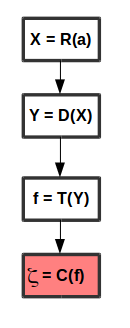
\includegraphics[width=0.75\textwidth]{ce1}
\end{minipage}
  \begin{minipage}{0.80\textwidth}
  \caption{$\textbf{pred}$ = $Model$($\textbf{a}$) }\label{exp:a2}
  \begin{algorithmic}[1]
    \Statex \textbf{Input :} $\textbf{a} \in \mathbb{R}^{12000.t}$
    \Statex \textbf{Output :} $\textbf{pred}$ \Comment{indices of predicted labels}
    \State $\textbf{C} = \textbf{a} \star {\textbf{W}_{STFT}}^{(256)}$ \Comment{$\textbf{C} \in \mathbb{R}^{512 \times P}, \textbf{W}_{STFT} \in \mathbb{R}^{512 \times 512}$}
    \State $\textbf{C} \leftarrow \textbf{C} \odot \textbf{C}$
    \State $\textbf{X} = \textbf{C} \star {\textbf{W}_{MEL}}^{(512)}$ \Comment{$\textbf{X} \in \mathbb{R}^{96 \times P}, \textbf{W}_{MEL} \in \mathbb{R}^{96 \times 512}$}
    \State $\textbf{X} \leftarrow ln(\textbf{X})$
    \State $\textbf{Y} = \textbf{X} \star {\textbf{W}_{MFCC}}^{(96)}$ \Comment{$\textbf{Y} \in  \mathbb{R}^{90 \times P}, \textbf{W}_{MFCC} \in \mathbb{R}^{90 \times 96}$}
    \State $\textbf{f} = BagOfFrames(\textbf{Y})$ \Comment{$\textbf{f} \in \mathbb{R}^{Z}$}
    \State $\bm{\zeta} = \sigma ({\color{red} \textbf{W}_{L2}} ReLU ({\color{red}\textbf{W}_{L1}}\textbf{f})) $ \Comment{$\bm{\zeta} \in \mathbb{R}^{63}, \textbf{W}_{L2} \in \mathbb{R}^{63 \times H}, \textbf{W}_{L1} \in \mathbb{R}^{H \times Z}$}
    \State $\textbf{pred} = \{ b(\zeta_{i}) | b(\zeta_{i}) = 1 \}$ \Comment{$ i \in \{1,2,..,63\}, b( \zeta_{i}) \in \{0,1\}$}
  \end{algorithmic}
  \end{minipage}
\end{algorithm}
\FloatBarrier

\noindent The network is trained with ADAM optimizer. The training settings that are used in this thesis were explained in Chapter 2, section \ref{training}. All ADAM parameters except the learning rate $\eta$ are used as proposed in  \cite{adam_o}. The learning rate can be different for different sections of the network and hence we differentiate the learning rate of the classifier with subscript $c$ ($\eta_{c}$). The learning rate is reduced by factor $\gamma_{c}$ every $step_{c}$ iterations. This is done because in the beginning, large learning rate is needed to approach the solution, but as the training approaches actual solution learning rate has to be reduced. Otherwise, the solution might be sub optimal. Even though the classifier is shallow, the network is fixed trained on the MTT dataset (source task) until convergence. The resulting weights are used as initialization for training on target dataset. Since our aim is to analyse only the CNNs, the training hyper-parameters values for the classifier are fixed with values shown in table \ref{tab:a2}.  

\begin{table}[H]
\label{tab:a2}
\centering
\begin{tabular}{| p{.3\textwidth} | p{.3\textwidth} | p{.3\textwidth} |}
\hline
\textbf{Hyper-parameter} & \textbf{Source task} & \textbf{Target task}\\
\hline
${\eta}_{c}$ & $1^{-2}$ & $1^{-3}$ \\ 
\hline
${\gamma}_{c}$ & $0.1$ & $ 0.1$\\
\hline
${step}_{c}$ & 10000 & 3000 \\
\hline
\end{tabular}
\caption{Training Hyper-Parameters for Classifier} 
\end{table}
\FloatBarrier

\noindent To set up a two layer neural network, the size of the classifier input (or feature) $Z$, the dimension of hidden layer $H$ and the size of the output $L$ should be known. The size of the output is equal to the number of labels in test. 63 labels are used for validation in target set. The experiments for different $H$ and $Z$ and their resulting WAUC scores are shown in table \ref{tab:a3}. (Here the features size ($Z$) resulting from the Bag of frames is equal to the number of cluster centres to be chosen)
 
\begin{table}[H]
\label{tab:a3}
\centering
\begin{tabular}{| p{.24\textwidth} | p{.24\textwidth}| p{.24\textwidth}| p{.24\textwidth} |}
\hline
& $H = \textbf{512}$ & $H = \textbf{1024}$ & $H = \textbf{2048}$\\
\hline
$Z = \textbf{512}$  & 0.63 & 0.64 & 0.63\\
\hline
$Z = \textbf{1024}$ & 0.64 & \textbf{0.67 }& 0.62\\ 
\hline
$Z = \textbf{2048}$ & 0.61 & 0.61 & 0.59\\
\hline
\end{tabular}
\caption{Hyper parameter search : Classifier hidden dimension (H), Feature dimension (Z)} 
\end{table}
\FloatBarrier

\noindent When the feature size is 512, it can be seen that the performance is capped around 0.64 for different hidden size. The performance improves with feature size 1024. However, the performance decreases when the dimension increases to 2048. This tells us that the model begins to over fit (learn the noisy data) when the number of parameters increases to 2048. Hence the feature dimension ($Z$) and hidden dimension ($H$) are fixed to \textbf{1024} for all the remaining analyses. 

\subsection{RNN Settings}
The error from classifier $C$ is back-propagated into the temporal approximation function $T$ with a 2 layer LSTM. Therefore, the Bag of frames algorithm is replaced with LSTM. The operators of LSTM $\bm{\Phi_{R1}}$ and $\bm{\Phi_{R2}}$ are solved to sequentially combine MFCC features from each STFT frame into a fixed size projection. The LSTM operators
\[
\bm{\Phi}_{Rj} = \{\textbf{W}_{(k,j)}, \textbf{U}_{(k,j)}\} \qquad k \in \{i,o,g,c\}, k \in \{1,2\}
\] 
were described in Chapter 2, section \ref{rnn}. Thus the learning is pushed into the temporal approximation function. But the number of STFT frames can be large for longer songs and the information at the beginning of sequence can get lost. To get around this problem, the first layer of LSTM is a \textit{sequence to one} network that combines frames up to 29.1s. The second layer of \textit{sequence to one} LSTM combines features from every 29.1s frame to a fixed sized projection. This computation is illustrated in step 6 - 12 of algorithm \ref{exp:a3}. There are 1366 STFT frames for 29.1s of 12 KHz sampled signal. Drop out with probability $p$ is used as the transition operation (referred in chapter 2, algorithm \ref{alg:2lstm}). Drop out acts as a regularizer that prevents the network from over-fitting.
\begin{algorithm}
\begin{minipage}{0.15\textwidth}
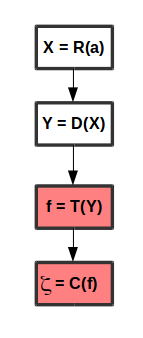
\includegraphics[width=0.75\textwidth]{ce2}
\end{minipage}
  \begin{minipage}{0.80\textwidth}
  \caption{$\textbf{pred}$ = $Model$($\textbf{a}$) }\label{exp:a3}
   {\fontsize{8}{0}
  \begin{algorithmic}[1]
    \Statex \textbf{Input :} $\textbf{a} \in \mathbb{R}^{12000.t}$
    \Statex \textbf{Output :} $\textbf{pred}$ \Comment{indices of predicted labels}
    \State $\textbf{C} = \textbf{a} \star {\textbf{W}_{STFT}}^{(256)}$ \Comment{$\textbf{C} \in \mathbb{R}^{512 \times P}, \textbf{W}_{STFT} \in \mathbb{R}^{512 \times 512}$}
    \State $\textbf{C} \leftarrow \textbf{C} \odot \textbf{C}$
    \State $\textbf{X} = \textbf{C} \star {\textbf{W}_{MEL}}^{(512)}$ \Comment{$\textbf{X} \in \mathbb{R}^{96 \times P}, \textbf{W}_{MEL} \in \mathbb{R}^{96 \times 512}$}
    \State $\textbf{X} \leftarrow ln(\textbf{X})$
    \State $F = 1366$
    \State $W = floor(\frac{P}{F})$
    \For{$i \in \{0,..,W\}$}
      \State $ \textbf{G} \leftarrow \textbf{X}[:,(i+1)F]$
      \State $\textbf{Y} \leftarrow \textbf{G} \star {\textbf{W}_{MFCC}}^{(96)}$ \Comment{$\textbf{Y} \in \mathbb{R}^{90 \times F}, \textbf{W}_{MFCC} \in \mathbb{R}^{90 \times 96}$}
      \State $\textbf{F}[i] = {Drop}_{(p)}(Seq2One\_LSTM(\textbf{Y} | {\color{red}\bm{\Phi}_{R2}} ))$ \Comment{$\textbf{F} \in \mathbb{R}^{T \times W}$}
    \EndFor
    \State $\textbf{f} = {Drop}_{(p)}(Seq2One\_LSTM(\textbf{F} | {\color{red}\bm{\Phi}_{R1}}))$ \Comment{$\textbf{f} \in \mathbb{R}^{1024}$}
    \State $\bm{\zeta} = \sigma ({\color{red} \textbf{W}_{L2}} ReLU ({\color{red}\textbf{W}_{L1}}\textbf{f})) $ \Comment{$\bm{\zeta} \in \mathbb{R}^{63}, \textbf{W}_{L2} \in \mathbb{R}^{63 \times 1024}, \textbf{W}_{L1} \in \mathbb{R}^{1024 \times 1024}$}
    \State $\textbf{pred} = \{ b(\zeta_{i}) | b(\zeta_{i}) = 1 \}$ \Comment{$ i \in \{1,2,..,63\}, b( \zeta_{i}) \in \{0,1\}$}
  \end{algorithmic}
  }
  \end{minipage}
\end{algorithm}
\FloatBarrier

\noindent To set up a 2 layer LSTM, the size of hidden projection $T$ and the drop-out probability $p$ have to be known. Training settings for source and target tasks are same as that of the classifier. WAUC scores for different  $p$ and $T$ are shown in table \ref{tabl:a4}.
\begin{table}[H]
\label{tabl:a4}
\centering
\begin{tabular}{| p{.24\textwidth} | p{.24\textwidth}| p{.24\textwidth}| p{.24\textwidth} |}
\hline
& $T = \textbf{512}$ & $T = \textbf{1024}$ & $T = \textbf{2048}$\\
\hline
$p = \textbf{0}$  & 0.66 & 0.61 & 0.59\\
\hline
$p = \textbf{0.3}$ & 0.68 & \textbf{0.74} & 0.68\\ 
\hline
$p = \textbf{0.5}$ & 0.67 & 0.71 & 0.64\\
\hline
\end{tabular}
\caption{Hyper parameter search : RNN hidden dimension (T), Drop-out probability (p)} 
\end{table}
\FloatBarrier

\noindent The optimum classifier settings from experiments in previous section is used ($H = Z = 1024$). The hidden dimension ($T$) 1024 is found to be optimal. It can be seen that the network over-fits without the drop-out ($p = 0$). Therefore, $p = 0.3$ and $T = 1024$ is used fixed for remaining analyses.

\subsubsection{Black-box LSTM}
\begin{minipage}{0.15\textwidth}
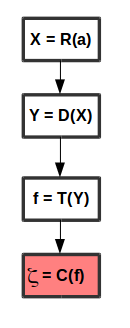
\includegraphics[width=0.75\textwidth]{ce1}
\end{minipage}
\begin{minipage}{0.80\textwidth}
The operators of LSTM trained on the source task can also be used as black-box feature extractor for the target task (that is, LSTM is not further trained with target data). Sometimes, fine-tuning on the target training set might degrade the operators. This could either be because of convergence of source task training towards general purpose features or because of in-sufficient training data in the target set. To check this, LSTM trained on the source dataset is used as a black-box feature extractor for the target task. But, for the optimal LSTM settings from experiments in previous section ($p = 0.3$, $T=1024$), WAUC drops to \textbf{0.65}. This shows that the source task features cannot be used as general purpose features and still needs task-dependent training. 
\end{minipage}

\subsection{CNN Settings}

\begin{algorithm}
\begin{minipage}{0.15\textwidth}
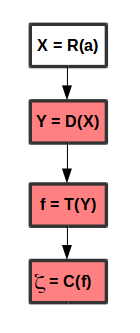
\includegraphics[width=0.75\textwidth]{ce3}
\end{minipage}
  \begin{minipage}{0.80\textwidth}
  \caption{$\textbf{pred}$ = $Model$($\textbf{a}$) }\label{exp:a4}
   {\fontsize{8}{0}
  \begin{algorithmic}[1]
    \Statex \textbf{Input :} $\textbf{a} \in \mathbb{R}^{12000.t}$
    \Statex \textbf{Output :} $\textbf{pred}$ \Comment{indices of predicted labels}
    \State $\textbf{C} = \textbf{a} \star {\textbf{W}_{STFT}}^{(256)}$ \Comment{$\textbf{C} \in \mathbb{R}^{512 \times P}, \textbf{W}_{STFT} \in \mathbb{R}^{512 \times 512}$}
    \State $\textbf{C} \leftarrow \textbf{C} \odot \textbf{C}$
    \State $\textbf{X} = \textbf{C} \star {\textbf{W}_{MEL}}^{(512)}$ \Comment{$\textbf{X} \in \mathbb{R}^{96 \times P}, \textbf{W}_{MEL} \in \mathbb{R}^{96 \times 512}$}
    \State $\textbf{X} \leftarrow ln(\textbf{X})$
    \State $F = 1366$
    \State $W = floor(\frac{P}{F})$
    \For{$i \in \{0,..,W\}$}
      \State $ \textbf{G} \leftarrow \textbf{X}[:,(i+1)F]$
      \State $\textbf{Y}[i] = CHOI\_CNN(\textbf{G} | {\color{red} \bm{\Phi}_{C}})$ \Comment{$\textbf{Y} \in \mathbb{R}^{1024 \times W}$}
     \EndFor
     \State $\textbf{F} = {Drop}_{(0.3)}(Seq2Seq\_LSTM(\textbf{Y} | {\color{red}\bm{\Phi}_{R2}} ))$ \Comment{$\textbf{F} \in \mathbb{R}^{1024 \times W}$}
    \State $\textbf{f} = {Drop}_{(0.3)}(Seq2One\_LSTM(\textbf{F} | {\color{red}\bm{\Phi}_{R1}}))$ \Comment{$\textbf{f} \in \mathbb{R}^{1024}$}
    \State $\bm{\zeta} = \sigma ({\color{red} \textbf{W}_{L2}} ReLU ({\color{red}\textbf{W}_{L1}}\textbf{f})) $ \Comment{$\bm{\zeta} \in \mathbb{R}^{63}, \textbf{W}_{L2} \in \mathbb{R}^{63 \times 1024}, \textbf{W}_{L1} \in \mathbb{R}^{1024 \times 1024}$}
    \State $\textbf{pred} = \{ b(\zeta_{i}) | b(\zeta_{i}) = 1 \}$ \Comment{$ i \in \{1,2,..,63\}, b( \zeta_{i}) \in \{0,1\}$}
  \end{algorithmic}
  }
  \end{minipage}
\end{algorithm}
\FloatBarrier

\begin{table}[H]
\label{tab:a5}
\centering
\begin{tabular}{| p{.40\textwidth} | p{.40\textwidth}| p{.15\textwidth}| }
\hline
$\textbf{Layer = 1,2}$ & $\textbf{Layer = 3,4,5}$ & \textbf{WAUC}\\
\hline
Freeze & $(1^{-3}; 30K)$ & 0.79\\
\hline
Freeze & $(1^{-3}; 50K)$ & \textbf{0.81}\\
\hline
Freeze & $(1^{-3}; 70K)$ & 0.74\\
\hline
Freeze & $(1^{-4}; 30K)$ & 0.79\\
\hline
Freeze & $(1^{-4}; 50K)$ & \textbf{0.81}\\
\hline
Freeze & $(1^{-4}; 70K)$ & 0.77\\
\hline
\end{tabular}
\caption{Source task experiments with 1st two layers freezed : $(\eta_{f}, {step}_{f})$} 
\end{table}

\begin{table}[H]
\label{tab:a6}
\centering
\begin{tabular}{| p{.40\textwidth} | p{.40\textwidth}| p{.15\textwidth}| }
\hline
$\textbf{Layer = 1,2}$ & $\textbf{Layer = 3,4,5}$ & \textbf{WAUC}\\
\hline
$(1^{-5}; 50K)$ & $(1^{-3}; 50K)$ & 0.82\\
\hline
$(1^{-5}; 50K)$ & $(1^{-4}; 50K)$ & 0.79\\
\hline
$(1^{-4}; 50K)$ & $(1^{-3}; 50K)$ & \textbf{0.84}\\
\hline
$(1^{-4}; 50K)$ & $(1^{-4}; 50K)$ & 0.77\\
\hline
$(1^{-4}; 70K)$ & $(1^{-3}; 50K)$ & 0.82\\
\hline
$(1^{-4}; 70K)$ & $(1^{-4}; 50K)$ & 0.79\\
\hline
$(1^{-3}; 50K)$ & $(1^{-3}; 50K)$ & 0.83\\
\hline
$(1^{-3}; 50K)$ & $(1^{-4}; 50K)$ & 0.76\\
\hline
$(1^{-3}; 70K)$ & $(1^{-3}; 50K)$ & 0.81\\
\hline
$(1^{-3}; 70K)$ & $(1^{-4}; 50K)$ & 0.76\\
\hline
\end{tabular}
\caption{Source task experiments with all layers trained : $(\eta_{f}, {step}_{f})$}
\end{table}

\begin{table}[H]
\label{tab:a7}
\centering
\begin{tabular}{| p{.40\textwidth} | p{.40\textwidth}| p{.15\textwidth}| }
\hline
$\textbf{Layer = 1,2}$ & $\textbf{Layer = 3,4,5}$ & \textbf{WAUC}\\
\hline
Freeze & $(1^{-3}; 5K)$ & 0.65\\
\hline
Freeze & $(1^{-3}; 10K)$ & 0.63\\
\hline
Freeze & $(1^{-3}; 20K)$ & 0.61\\
\hline
Freeze & $(1^{-4}; 5K)$ & 0.67\\
\hline
Freeze & $(1^{-4}; 10K)$ & \textbf{0.68}\\
\hline
Freeze & $(1^{-4}; 20K)$ & 0.63\\
\hline
\end{tabular}
\caption{Target task experiments with 1st two layers freezed : $(\eta_{f}, {step}_{f})$} 
\end{table}

\begin{table}[H]
\label{tab:a8}
\centering
\begin{tabular}{| p{.40\textwidth} | p{.40\textwidth}| p{.15\textwidth}| }
\hline
$\textbf{Layer = 1,2}$ & $\textbf{Layer = 3,4,5}$ & \textbf{WAUC}\\
\hline
$(1^{-6}; NA)$ & $(1^{-4}; 10K)$ & 0.64\\
\hline
$(1^{-5}; 10K)$ & $(1^{-4}; 10K)$ & \textbf{0.71}\\
\hline
$(1^{-5}; 20K)$ & $(1^{-4}; 10K)$ & 0.69\\
\hline
$(1^{-4}; 10K)$ & $(1^{-4}; 10K)$ & 0.68\\
\hline
$(1^{-4}; 20K)$ & $(1^{-4}; 10K)$ & 0.67\\
\hline
\end{tabular}
\caption{Target task experiments with all layers trained : $(\eta_{f}, {step}_{f})$}
\end{table}

\subsubsection{Black-box CNN + Fine-tune LSTM}
\begin{minipage}{0.15\textwidth}
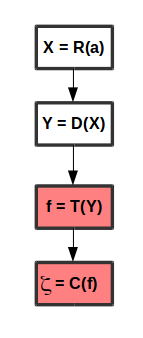
\includegraphics[width=0.75\textwidth]{ce2}
\end{minipage}
\begin{minipage}{0.80\textwidth}
Text goes here
\end{minipage}

\subsubsection{Black-box CNN + Black-box LSTM}
\begin{minipage}{0.15\textwidth}
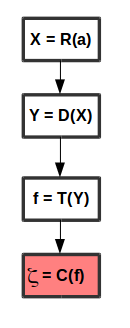
\includegraphics[width=0.75\textwidth]{ce1}
\end{minipage}
\begin{minipage}{0.80\textwidth}
Text goes here
\end{minipage}

\subsubsection{Black-box CNN + Bag of Frames}
\begin{minipage}{0.15\textwidth}
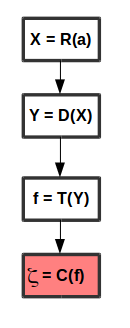
\includegraphics[width=0.75\textwidth]{ce1}
\end{minipage}
\begin{minipage}{0.80\textwidth}
Text goes here
\end{minipage}

\subsection{Analyses of Convolution Neural Networks}
\label{pretrained}

\subsubsection{Fine-tune CNN + Fine-tune LSTM}


In Chapter 2 (ref. \ref{stacked}), it was shown how Convolution Neural Networks (CNN) are motivating to be used as feature extractor for music signal. In Chapter 3 (ref. \ref{convolution}) some of the successful mel-spectrogram convolution architectures trained on MTT dataset showing state-of-art performance were discussed. Now we would like to see if such features extracted through these models can be used for auxiliary tasks. That is to say, the learned CNN parameters (weights) from \textit{source} dataset are used as initialization setting for \textit{target} tasks.    
\bigskip

\noindent The CNN architecture from \cite{choi_cnn} achieves the best AUC score on MTT dataset and hence this architecture is used for feature extraction. The algorithm for their model ($CHOI\_CNN$) is explained in section \ref{convolution} (Algorithm \ref{alg:choicnn}). The input to their CNN was 29.1s mel-spectrogram with representation parameters mentioned above (Thus resulting in 1366 time samples). So for our task, features are extracted every 29.1s and sequentially sent to RNN. The temporal summarization is done by 2 layer \textit{Long Short-Term Memory Recurrent Neural Network} (ref. \ref{rnn}). The RNN module does sequence to one mapping ($Seq2One$) of the input features. This entire model is then trained for 150K iteration on MTT dataset with top 50 tags. Their model was already trained on Million Song Dataset \cite{MSD} with top 50 \textit{Last.fm} tags. We just fine-tune their model on MTT dataset after merging clips from same song. Features of clips from same song are sequentially given as input to RNN with a dropout (ref. \ref{training}) of 0.3 after each layer, which then projects to a fixed sized feature vector. The output of RNN is then passed to a fully connected layer with 50 output units and \textit{sigmoid} activation. ADAM optimizer with \textit{binary-cross-entropy} loss function is used for training. The starting learning rate is $0.001$, decaying at $1^{-8}$ and beta $0.99$ (ref. \ref{training}). Algorithm for $L$ labels is described below and the notations used are consistent with formalisms in Chapter \ref{Chapter2}. The algorithm is implemented in \textit{Torch} [torch] and mel-spectrogram was extracted using \textit{Librosa} [librosa]
\bigskip 

\begin{algorithm}
  \caption{$Pred$ = MODEL($\textbf{a}$) }
  \label{alg:cnnrnn}
  {\fontsize{1}{0}
  \begin{algorithmic}[1]
    \Statex \textbf{Input :} $\textbf{a} \in \mathbb{R}^{N}$
    \Statex \textbf{Output :} $Pred \in \mathbb{R}^{L}$ 
    \State $\textbf{C} = STFT(\textbf{a})$ \Comment{$\textbf{C} \in \mathbb{C}^{M \times P}$}
    \State $\textbf{Y}_{r} = Log(\textbf{C} \odot \textbf{C})$ \Comment{$\textbf{Y}_{r} \in \mathbb{R}^{M \times P}$}
    \State $\textbf{R} = MEL(\textbf{Y}_{r})$ \Comment{$\textbf{R} \in \mathbb{R}^{96 \times P}$}
    \State $W = floor(\frac{P}{1366})$
    \For{$i \in \{0,..,W\}$}
      \State $\textbf{X} \leftarrow \textbf{R}[:][i:(i+1).1366]$ \Comment{$\textbf{X} \in \mathbb{R}^{96 \times 1366}$}
      \State $\textbf{Y}[i] \leftarrow CHOI\_CNN(\textbf{X})$ \Comment{$\textbf{Y} \in \mathbb{R}^{1024 \times W}$} 
    \EndFor
    \State $\textbf{Y}_{1} = Drop_{(0.3)}(Seq2Seq\_LSTM(\textbf{Y}))$ \Comment{$\textbf{Y}_{1} \in \mathbb{R}^{1024 \times W}$}
    \State $\textbf{y}_{2} = Drop_{(0.3)}(Seq2One\_LSTM(\textbf{Y}_{1}))$ \Comment{$\textbf{y}_{2} \in \mathbb{R}^{1024}$}
    \State $Pred = \sigma(L(\textbf{W})\textbf{y}_{2}))$ \Comment{$\textbf{W} \in \mathbb{R}^{L \times 1024}$}
  \end{algorithmic}
  }
\end{algorithm}
\FloatBarrier

\noindent This CNN model can either be used as a \textit{black-box} feature extractor (That is, weights of the model are not modified while training the \textit{target-task}) or certain layers can be \textit{fine-tuned} (That is, we continue the training on \textit{target-task}). Both the cases are looked separately,
\bigskip

\noindent \textbf{Blackbox CNN + RNN :}\\ 
The weights of CNN trained on the source task are not modified (no fine-tuning). The weights of RNN are also initiazied with those trained on source task. The fully-connected layer in the source task is changed to 65 output units. (i.e 65 labels). The network is trained by back-propagating through the fully connected layer and RNN with \textit{binary-cross entropy} loss function (ref. \ref{training}). The optimization parameters are same as that of \textit{source task}. Training is stopped after 25K iterations, after which the model begins to over-fit. Weighted averaged AUC (WAUC) was \textbf{0.65}
\bigskip

\noindent \textbf{Fine-tune CNN + RNN :}\\
With the same parameter settings, the last layer of CNN was finetuned after 5K iterations. Training was then continued until 25K iterations and WAUC went up to \textbf{0.69}. When last two CNN layers were finetuned WAUC further improved to \textbf{0.71}. Fine-tuning earlier layers proved sub-optimal. 
\bigskip

\noindent This tells us that in the final layers CNN tend to find features specific to task. (Recalling that labels for source and target tasks are different). However, we still do not know if convolutions over mel-spectrogram will be better than MFCCs which is proven to model audio discriminants. Before going there, the effectiveness of RNN should also be questioned. It was hypothesised in Chapter 3 (\ref{model}) that Bag-of-Frames (\ref{clustering}) features using K-Means (which was actually used in \cite{MultiScale} to attain state of art performance) may not be suitable for summarizing features for longer audio. So we test this by replacing RNN with Bag Of Frames (BoF) features.
\bigskip

\noindent \textbf{CNN + BoF :}
The CNN is first finetuned for 10K iterations with algorithm \ref{alg:cnnrnn}. Then 1024 centroids of CNN features are found by unsupervised training on both MTT and our target dataset. This is followed by multi layer perceptron with a hidden layer of 512 units and ReLU activation. Having hidden size of 1024 did not improve the result. WAUC was \textbf{0.67}. The algorithm is described below,

\begin{algorithm}
  \caption{$Pred$ = MODEL($\textbf{a}$) }\label{alg:cnnbow}
  \begin{algorithmic}[1]
    \Statex \textbf{Input :} $\textbf{a} \in \mathbb{R}^{N}$
    \Statex \textbf{Output :} $Pred \in \mathbb{R}^{65}$ 
    \State $\textbf{C} = STFT(\textbf{a})$ \Comment{$\textbf{C} \in \mathbb{C}^{M \times P}$}
    \State $\textbf{Y}_{r} = Log(\textbf{C} \odot \textbf{C})$ \Comment{$\textbf{Y}_{r} \in \mathbb{R}^{M \times P}$}
    \State $\textbf{R} = MEL(\textbf{Y}_{r})$ \Comment{$\textbf{R} \in \mathbb{R}^{96 \times P}$}
    \State $W = floor(\frac{P}{1366})$
    \For{$i \in \{0,..,W\}$}
      \State $\textbf{X} \leftarrow \textbf{R}[:][i:(i+1).1366]$ \Comment{$\textbf{X} \in \mathbb{R}^{96 \times 1366}$}
      \State $\textbf{Y}[i] \leftarrow CHOI\_CNN(\textbf{X})$ \Comment{$\textbf{Y} \in \mathbb{R}^{1024 \times W}$} 
    \EndFor
    \State $\textbf{y}_{1} = BagOfFrames(\textbf{Y},1024)$ \Comment{$\textbf{y}_{1} \in \mathbb{R}^{1024}$}
     \State $Pred = \sigma(L(\textbf{W}_{2})ReLU(L(\textbf{W}_{1})\textbf{y}_{1}))$ \Comment{$\textbf{W}_{2} \in \mathbb{R}^{65 \times 512}, \textbf{W}_{1} \in \mathbb{R}^{512 \times 1024}$}
  \end{algorithmic}
\end{algorithm}
\FloatBarrier
    
\subsection{Comparision of MFCC with CNN features}    
\label{mfcc}  
MFCCs are still de-facto standard for classifications on small datasets. If CNNs had to outperform MFCCs, the learned parameters should have to encode discriminants similar to MFCCs. MFCCs are computed by taking discrete-cosine transform on log mel-spectrogram (ref. \ref{basis}). Following the comparison strategies from \cite{choi_cnn}, we retain 30 coefficients, their first and second derivative, resulting in a vector of size 90 for each STFT frame.
\bigskip

\noindent \textbf{MFCC + RNN :}\\
Now, MFCCs from every STFT window is passed in a \textit{30s  Batched sequence} to a Sequence to one LSTM, which results in a projection for every 30s window. These sequence of 30s frames are then passed to another Sequence to One LSTM to get a final projection. This is done because a MFCCs from STFT frame will result in a long sequence and RNNs tend to forget the information in the earlier sequence samples. This network was first trained with MTT dataset before our target dataset. The parameter setting are same as those used while training \textbf{CNN+RNN}. The resulting WAUC was \textbf{0.74}   
\begin{algorithm}
  \caption{$Pred$ = MODEL($\textbf{a}$) }\label{alg:mfccrnn}
  \begin{algorithmic}[1]
    \Statex \textbf{Input :} $\textbf{a} \in \mathbb{R}^{N}$
    \Statex \textbf{Output :} $Pred \in \mathbb{R}^{65}$ 
    \State $\textbf{R} = MFCC(\textbf{a})$ \Comment{$\textbf{R} \in \mathbb{R}^{90 \times P}$}
        \State $W = floor(\frac{P}{1366})$
    \For{$i \in \{0,..,W\}$}
      \State $\textbf{X} \leftarrow \textbf{R}[:][i:(i+1).1366]$ \Comment{$\textbf{X} \in \mathbb{R}^{90 \times 1366}$}
    \State $\textbf{Y}[i] \leftarrow Drop_{(0.3)}(Seq2One\_LSTM(\textbf{X}))$ \Comment{$\textbf{Y} \in \mathbb{R}^{1024 \times W}$}
    \EndFor
    \State $\textbf{y} = Drop_{(0.3)}(Seq2One\_LSTM(\textbf{Y}))$ \Comment{$\textbf{y} \in \mathbb{R}^{1024}$}
    \State $Pred = \sigma(L(\textbf{W})\textbf{y}))$ \Comment{$\textbf{W} \in \mathbb{R}^{65 \times 1024}$}
  \end{algorithmic}
\end{algorithm}
\FloatBarrier

\noindent \textbf{MFCC + BoF :}\\
RNN is repalaced with Bag of Frames features. Now WAUC drops to \textbf{0.62}
\begin{algorithm}
  \caption{$Pred$ = MODEL($\textbf{a}$) }\label{alg:mfccbow}
  \begin{algorithmic}[1]
    \Statex \textbf{Input :} $\textbf{a} \in \mathbb{R}^{N}$
    \Statex \textbf{Output :} $Pred \in \mathbb{R}^{65}$ 
    \State $\textbf{R} = MFCC(\textbf{a})$ \Comment{$\textbf{R} \in \mathbb{R}^{90 \times P}$}
   \State $\textbf{y} = BagOfFrames(\textbf{R},1024)$ \Comment{$\textbf{y} \in \mathbb{R}^{1024}$}
     \State $Pred = \sigma(L(\textbf{W}_{2})ReLU(L(\textbf{W}_{1})\textbf{y}))$ \Comment{$\textbf{W}_{2} \in \mathbb{R}^{65 \times 512}, \textbf{W}_{1} \in \mathbb{R}^{512 \times 1024}$}
  \end{algorithmic}
\end{algorithm}
\FloatBarrier    

\section{Summary of Results}
\label{results}
Summary of results is shown in the table below. It is seen that \textit{transfer learning} of convolutions over mel-spectrogram with architecture in \cite{choi_cnn}  cannot match with MFCCs for small datasets. This indicates that convolutional features from source dataset are more task-specific. It is also seen that \textit{Recurrent Neural Networks} perform better in summarizing features for longer audio. This indicates the existence of rhythmic patterns that discriminate music. 

   \begin{tabular}{ | p{5cm} | l |}
    \hline
    \textbf{Model} & \textbf{AUC} \\ \hline
    Finetune CNN + RNN &  0.71\\ \hline
    CNN + BoF  &  0.67\\ \hline
    MFCC + RNN &  \textbf{0.74} \\ \hline
    MFCC + BoF &  0.62 \\ \hline
    \hline
    \end{tabular}

